\documentclass[12pt,a4paper]{article}

% --- Encoding and fonts ---
\usepackage[utf8]{inputenc}
\usepackage[T1]{fontenc}
\usepackage{mathptmx} % Times-like font

% --- Page layout ---
\usepackage[margin=2.5cm]{geometry}
\usepackage{setspace}
\doublespacing

% --- Language ---
\usepackage[english]{babel}

% --- Tables and figures ---
\usepackage{booktabs}
\usepackage{tabularx}
\usepackage{multirow}
\usepackage{array}
\usepackage{graphicx}
\usepackage{float}

% --- References ---
\usepackage[style=apa,backend=biber,sortcites=true,sorting=nyt]{biblatex}
\addbibresource{references.bib}

% --- Hyperlinks ---
\usepackage[colorlinks=true,linkcolor=blue,citecolor=blue,urlcolor=blue]{hyperref}

% --- TikZ and pgfplots ---
\usepackage{tikz}
\usepackage{pgfplots}
\pgfplotsset{compat=1.18}
\usetikzlibrary{arrows.meta,positioning,calc}

% --- Miscellaneous ---
\usepackage{csquotes}
\usepackage{enumitem}
\usepackage{xcolor}

% --- Title block ---
\title{\textbf{Beyond Video Slop: A Multi-Format Framework for Understanding AI-Generated Content Pollution}}
\author{%
  Jiyeon Yoon\\
  \textit{Independent Researcher}\\
  \texttt{heznpc@gmail.com}%
}
\date{}

\begin{document}

\maketitle

% ============================================================
% ABSTRACT
% ============================================================
\begin{abstract}
\noindent
The public and scholarly discourse on AI-generated low-quality content---commonly termed ``slop''---is dominated by video. The shutdown of OpenAI's Sora, YouTube's anti-slop campaign, and reports of children's feeds contaminated with synthetic video have captured attention. Yet video is neither the most pervasive nor the most damaging form of AI slop. This paper proposes the AI-Generated Multi-Format Slop Model (AMSM), a five-dimensional framework for analyzing slop across all content formats: video, text, card news/infographics, fake reviews, academic papers, news articles, audio, and books. The five dimensions---Production Cost Asymmetry, Detection Difficulty Index, Ecosystem Damage Potential, Algorithmic Amplification Susceptibility, and Regulatory Coverage Gap---enable systematic cross-format comparison. Applying AMSM reveals two novel findings. First, the Production--Detection Paradox: research investment is inversely correlated with actual threat level, as the most-studied format (video) is the most detectable, while the least-studied formats (text, hybrid card news) are the hardest to detect and cause the greatest damage. Second, the Algorithm--Slop Co-evolution Model: platform algorithms do not merely distribute slop but co-evolve with it through a four-stage feedback loop that can be empirically tested through ongoing natural experiments. The paper concludes with a concrete research agenda of seven testable hypotheses, prioritized by feasibility and impact, for a research community that has been looking at only one corner of a much larger problem.

\medskip
\noindent\textbf{Keywords:} AI slop, generative AI, content moderation, platform algorithms, multi-format framework, detection asymmetry, information pollution
\end{abstract}

\newpage

% ============================================================
% 1  INTRODUCTION
% ============================================================
\section{Introduction}

On March 24, 2026, OpenAI announced the shutdown of Sora, its viral AI video generation app. At its peak in November 2025, Sora had reached 3.3 million monthly downloads. By February 2026, usage had collapsed to 1.1 million, and OpenAI---pivoting toward its Q4 2026 IPO---pulled the plug entirely \parencite{NPR2026a}. The following day, Disney's planned billion-dollar investment and licensing deal collapsed, with no funds having been transferred. NPR summarized the moment: ``Sora is going away, but its legacy will be the spread of AI video slop'' \parencite{NPR2026b}.

The Sora shutdown was the symbolic endpoint of a turbulent period. In December 2025, Merriam-Webster named ``slop'' its word of the year, defining it as ``low-quality digital content mass-produced through artificial intelligence.'' YouTube's CEO declared slop reduction his top priority for 2026. By March, YouTube was asking users directly: ``Does this feel like AI slop?'' \parencite{Dexerto2026}. Instagram head Adam Mosseri announced a strategic shift toward prioritizing authentic content, stating that ``authenticity is becoming infinitely reproducible'' \parencite{Mosseri2025}. The extent to which this has been implemented as a concrete algorithmic change remains unconfirmed. Reddit introduced human verification via passkeys to combat bot accounts \parencite{WinBuzzer2026}. The backlash was real, measurable, and overwhelmingly focused on one thing: video.

This focus is understandable. The Kapwing AI Slop Report \parencite{Kapwing2025}, the most comprehensive empirical study to date, analyzed 15,000 trending YouTube channels and found 278 dedicated AI slop channels with 63 billion cumulative views, 221 million subscribers, and an estimated \$117 million in annual ad revenue. Between 21\% and 33\% of content shown to new YouTube users was AI-generated slop or ``brainrot.'' A \textit{New York Times} investigation reported that approximately 40\% of video recommended to children was AI-generated \parencite{NYT2026}. These numbers are alarming.

But they describe only one format.

Simultaneously---and with far less attention---AI slop was saturating every other content format on the internet. An Ahrefs analysis of 900,000 newly published web pages found that 74.2\% contained AI-generated content (pure AI 2.5\% + human--AI mix 71.7\%) \parencite{Ahrefs2025}. Separately, a Graphite study estimated that approximately 52\% of English articles show AI involvement \parencite{Graphite2025}. Originality.AI reported that AI content in Google's top 20 search results had risen from 2.27\% in 2019 to 19.56\% in 2025. Over 54\% of LinkedIn long-form posts were estimated to be AI-generated \parencite{OriginalityAI2025a}. NewsGuard identified 1,265 partisan-funded ``pink slime'' news sites \parencite{NewsGuard2024}, with a separate category of 3,006 AI content farm sites identified by October 2025. Spotify removed 75 million spam tracks in twelve months \parencite{NME2025}. Wiley retracted 11,300 academic papers from Hindawi journals due to paper mill infiltration, shuttering 19 journals and abandoning the Hindawi brand entirely \parencite{TheRegister2024}. On Amazon, one Korean publisher produced 9,000 AI-generated books in a single year \parencite{KoreaTimes2025}. And on Instagram and Naver, AI-generated card news---a hybrid image-text format with zero detection research---was being produced at a rate of 100 posts in five minutes using ChatGPT and Canva's bulk creation feature \parencite{Lee2025}.

The scholarly literature reflects the same video-centrism. Deepfake detection research comprises thousands of papers with established benchmarks such as FaceForensics++ and the Deepfake Detection Challenge. AI video slop has received dedicated empirical studies \parencite{Jones2025,Kapwing2025}. But text-specific slop research amounts to essentially one paper---\textcite{Shaib2025}'s ``Measuring AI Slop in Text.'' Card news and infographic slop have received no academic attention whatsoever. The detection research landscape for hybrid image-text formats is, as documented in a comprehensive survey of the field, ``virtually nonexistent'' (see Section~\ref{sec:framework}).

This paper argues that the video-centric framing of AI slop is not merely incomplete---it is actively misleading. It directs research attention, platform resources, and regulatory action toward the format that is, by several measurable dimensions, among the least threatening. Meanwhile, formats with higher production scalability, greater detection difficulty, more severe downstream harm, and weaker regulatory coverage operate largely unexamined.

To address this, I propose the AI-Generated Multi-Format Slop Model (AMSM): a unified, five-dimensional framework for comparing AI slop across all content formats. AMSM enables two novel analyses. First, the Production--Detection Paradox, which demonstrates that research investment is inversely correlated with actual threat. Second, the Algorithm--Slop Co-evolution Model, which reconceptualizes the relationship between platform algorithms and slop production as a dynamic feedback system rather than a one-directional distribution pipeline.

The paper proceeds as follows. Section~\ref{sec:literature} reviews the existing literature, organizing it by definitional work, empirical studies, detection research, and platform/regulatory responses, and identifies three systematic gaps. Section~\ref{sec:framework} presents the AMSM framework in detail, with a comprehensive cross-format comparison table. Section~\ref{sec:paradox} develops the Production--Detection Paradox. Section~\ref{sec:coevolution} introduces the Algorithm--Slop Co-evolution Model. Section~\ref{sec:agenda} proposes a research agenda of seven testable hypotheses. Section~\ref{sec:implications} discusses implications for platforms, regulators, researchers, and the public. Section~\ref{sec:limitations} addresses limitations. Section~\ref{sec:conclusion} concludes.

A shorter commentary focusing specifically on the production-detection asymmetry and its implications for research prioritization and governance is available as a companion piece \parencite{author2026pda}.

A note on positionality: the author is an independent developer, not an academic. This vantage point provides direct familiarity with the tools, pipelines, and economics of AI content production that inform the production cost estimates and automation analyses throughout this paper. Where practitioner knowledge is used, it is clearly noted.


% ============================================================
% 2  LITERATURE REVIEW
% ============================================================
\section{Literature Review}
\label{sec:literature}

\subsection{Defining AI Slop}

The term ``slop'' entered widespread use in 2024--2025, but the academic community has yet to converge on a single definition. Three strands of definitional work can be identified.

The first is \emph{typological}. \textcite{MadsenPuyt2025} proposed the 7Vs of AI Slop: Volume (near-zero marginal cost mass production), Velocity (real-time generation and distribution), Variety (spanning text, image, video, audio, and beyond), Value (cultural and epistemic value erosion), Verification (absence of fact-checking), Visibility (algorithmic amplification), and Virality (optimization for memetic spread). They argue that AI slop is ``not a passing nuisance but a structural feature of contemporary media ecologies'' and characterize major platforms as ``industrial slop farms'' where ``monetization programs actively reward volume over value.'' The 7Vs framework is valuable for its comprehensiveness but remains descriptive; it does not provide operationalizable metrics for cross-format comparison.

The second strand is \emph{anatomical}. In discussions of academic publishing quality, a recurring descriptive categorisation has emerged under the acronym SLOP: Shallow analysis, Low-quality execution, Overgeneralized claims, and Poorly-sourced citations. This framework is precise but domain-specific, designed for scholarly content and not readily transferable to other formats.

The third strand is \emph{philosophical}. \textcite{Kommers2025}, working from the MINT Research Lab at institutions including the Alan Turing Institute and Cornell, identified three ``prototypical properties'' of slop: superficial competence (expert-level surface quality masking the absence of genuine communicative intent), asymmetric effort (production requiring dramatically less effort than traditional creation), and mass producibility (optimization for large-scale generation within digital ecosystems). They further proposed four normative objections to slop: epistemic pollution, automation bias, illegitimate reason-giving, and nonconsensual imposition. Their working definition---descriptively, model-generated content that appears competent but is factually uncertain, conceptually generic, and responsively hollow, produced at low cost through engagement-optimized distribution pathways; normatively, objectionable when it predictably degrades the epistemic environment through noise accumulation, trust signal erosion, and quality displacement---is the most rigorous available but has not been empirically validated.

Additionally, \textcite{Shaib2025} provided the first measurement framework for text slop specifically, identifying three evaluative dimensions through expert interviews: Information Quality (factual errors, biased language), Information Utility (redundancy, lack of depth), and Style Quality (verbosity, flattery, genericity). Their finding that ``binary slop judgments are somewhat subjective, but such determinations nonetheless correlate with latent dimensions such as coherence and relevance'' suggests that slop, while partially subjective, is amenable to systematic measurement.

What none of these frameworks provides is a mechanism for comparing slop \emph{across} formats. The 7Vs describe what slop is; the SLOP Anatomy describes how it manifests in one domain; \textcite{Kommers2025} describe why it matters normatively; \textcite{Shaib2025} describe how to measure it in text. The AMSM framework proposed in Section~\ref{sec:framework} is designed to fill this gap.

\subsection{Empirical Studies}

Empirical research on AI slop is growing but remains concentrated in video. The Kapwing Report \parencite{Kapwing2025} analyzed 15,000 trending YouTube channels across all countries and identified 278 AI slop channels with 63 billion cumulative views. South Korea led with 8.45 billion views across 11 channels---1.6 times the second-place country, Pakistan (5.34 billion). A new-account experiment found 21\% of the first 500 recommended Shorts were AI-generated, rising to 33\% when including ``brainrot'' content. Notably, slop was absent from the first 16 recommended videos, appearing only after the algorithm began optimizing---suggesting algorithmic amplification rather than baseline presence.

\textcite{Jones2025}, published in \textit{JMIR Medical Education}, conducted the first peer-reviewed empirical study, analyzing 1,082 biomedical education videos. They found a 5.3\% slop rate, with 78.7\% of slop concentrated in YouTube Shorts despite Shorts comprising only 34.3\% of their sample. A critical finding: ``None of the metrics we collected correlates significantly with the presence of slop''---standard engagement metrics could not distinguish slop from legitimate content.

\textcite{Moller2026}, published in \textit{Nature Scientific Reports}, conducted a controlled experiment with 680 US participants and found that AI tools create a ``complex duality'': increasing content volume and engagement while simultaneously decreasing perceived quality and authenticity. Most importantly, they identified a ``negative spill-over effect''---AI content in a discussion degraded the quality of contributions from participants who were not using AI tools.

For non-video formats, empirical data comes primarily from industry sources. Originality.AI tracked AI content in Google search results growing from 2.27\% (2019) to 19.56\% (2025). In academic publishing, a study published in \textit{Nature Human Behaviour} found that 22.5\% of sentences in computer science paper abstracts show LLM modification \parencite{Liang2025}; the original authors explicitly noted they did not estimate the proportion of fully AI-generated papers. The ``tortured phrases'' phenomenon---where LLMs replace standard terms with bizarre synonyms such as ``linear regression'' becoming ``straight relapse''---has been tracked across 7,500 registered phrases flagging over 20,000 papers \parencite{ProblematicPaperScreener2025}. PubMed analyses detected ChatGPT-characteristic terms such as ``delve'' increasing 654\% between 2020 and 2023 \parencite{SciAm2026}. In music, Spotify's removal of 75 million spam tracks and a fraud case involving AI-generated songs netting \$8 million through bot-driven streams illustrate the economic scale \parencite{Time2026}. In reviews, Originality.AI found that 3\% of Amazon bestseller reviews were AI-generated, with a systematic 5-star bias (74\% vs.\ 59\% for human reviews) \parencite{OriginalityAI2025b}.

\subsection{Detection Research: A Modality-Stratified Landscape}

Detection capabilities vary dramatically across content modalities, creating what I formalize in Section~\ref{sec:paradox} as the Production--Detection Paradox.

\textbf{Video} detection is the most mature field. On the FaceForensics++ benchmark, top models achieve AUROC of 91--97\% in-domain, degrading to 70--87\% cross-dataset (DFDC benchmark). For AI-generated video specifically (Sora, Runway, Kling), detection rates range from 85--94\%. Detection is aided by physical grounding violations---AI video must simulate gravity, inertia, and optics, producing artifacts that accumulate across frames.

\textbf{Audio} detection is similarly advanced. ASVspoof~5 challenge results show a best equal error rate (EER) of 2.59\% in the Open Condition (Team T45). Independent research using hybrid CNN+LSTM+GRU architectures has achieved EER of 0.0013, though this result was not part of the challenge itself. Commercial tools such as Resemble AI DETECT-2B achieve 94--98\% accuracy across 30+ languages. Audio detection benefits from acoustic signature analysis: synthetic speech carries frequency-domain artifacts that, while increasingly subtle, remain detectable with spectral analysis.

\textbf{Text} detection presents a starkly different picture. In controlled conditions, tools such as GPTZero report 88--95\% accuracy. But independent evaluations reveal severe fragility. Under adversarial paraphrasing attacks, detection performance degrades dramatically. \textcite{Krishna2023} showed that an 11B-parameter paraphraser drops DetectGPT accuracy from 70.3\% to 4.6\% at 1\% false positive rate. \textcite{Cheng2025} demonstrated an average 87.88\% reduction in true positive rate at 1\% FPR across eight detectors using a training-free adversarial paraphrasing attack. A reinforcement learning-based paraphrase policy \parencite{Ranganath2026} pushed mean AUROC from 0.789 to 0.432 with a 97.6\% attack success rate, and the attacks transferred to unseen detectors, indicating a structural rather than tool-specific vulnerability. For non-native English speakers, false positive rates reach 61.3\% \parencite{Liang2023}, meaning that the tools reliably flag legitimate ESL writing as AI-generated. KatFishNet \parencite{Park2025} improved Korean-language text detection by 19.78\% AUROC over baselines using Korean-specific linguistic features (spacing patterns, POS diversity, comma usage), but was evaluated only on 4 LLMs across 3 genres with no adversarial conditions.

\textbf{Image} detection occupies a middle ground: 88--97\% accuracy in benchmarks, degrading 15--35\% under real-world conditions (resizing, compression, screenshots). Human accuracy at detecting AI images is 49--61\%---effectively coin-flip level.

Most critically, \textbf{hybrid image-text formats} (card news, infographics, carousel posts) have never been evaluated. No detection tool is designed for them. No benchmark exists. No academic paper addresses the problem. As documented in a systematic review: ``AI-generated infographic/card news automatic detection has virtually no scholarly literature'' (see Section~\ref{sec:framework} for full analysis). This is the most consequential gap in the entire detection landscape.

\subsection{Platform and Regulatory Responses}

Platform responses have been primarily reactive and video-focused. YouTube's CEO declared slop reduction a 2026 priority and introduced a user feedback mechanism asking ``does this feel like AI slop?'' \parencite{Dexerto2026}. Instagram head Adam Mosseri announced a strategic shift toward prioritizing authentic content \parencite{Mosseri2025}. The extent to which this has been implemented as a concrete algorithmic change remains unconfirmed. Reddit implemented human verification through passkeys and biometric authentication \parencite{WinBuzzer2026}. TikTok introduced ``Manage Topics'' allowing users to control AI content exposure.

Regulatory frameworks are converging but remain incomplete. China's AI Content Labeling Measures (effective September 2025) represent the strongest enforcement: 37,000 non-compliant videos purged, 3,400 accounts suspended, 600,000 videos labeled. The EU AI Act's Article~50 transparency provisions are expected to take effect in August 2026. South Korea's AI Basic Act (effective January 2026) mandates watermark or written disclosure for AI content, with 5$\times$ punitive damages for harm. The United States has no federal law; California's SB~942 is expected in August 2026.

Critically, all of these measures disproportionately target audiovisual content. Text-based slop (blog posts, reviews, comments), hybrid formats (card news, infographics), and academic slop fall through coverage gaps. The FTC's fake review rule (effective October 2024, \$51,744 per violation) is an exception---but enforcement has been limited to 10 warning letters by December 2025 \parencite{FTC2024}.

\subsection{Identifying the Gap}

Three systematic blind spots emerge from this review:

\begin{enumerate}[leftmargin=*]
  \item \textbf{Video-centrism}: The majority of slop research, platform action, and regulatory effort targets video, despite text-based formats having demonstrably higher penetration rates (74.2\% of new web pages vs.\ 5.3--33\% of video feeds).

  \item \textbf{No cross-format comparison}: Each format is studied in isolation. No existing framework enables researchers to compare AI slop across formats on unified, operationalizable dimensions.

  \item \textbf{Hybrid-format neglect}: Card news, infographics, and carousel posts---formats that dominate engagement metrics on platforms such as Instagram and Naver---have received zero detection research, zero prevalence studies, and zero quality benchmarks.
\end{enumerate}

The AMSM framework addresses all three gaps.


% ============================================================
% 3  THE AMSM FRAMEWORK
% ============================================================
\section{The AMSM Framework}
\label{sec:framework}

\subsection{Design Rationale}

The AI-Generated Multi-Format Slop Model (AMSM) extends the 7Vs framework \parencite{MadsenPuyt2025} from description to operationalization. Where the 7Vs characterize what AI slop is, AMSM provides a mechanism for comparing it across formats by defining five measurable dimensions, each rated on a 1--5 scale with explicit criteria and supporting evidence.

AMSM is designed to be format-agnostic: its dimensions apply equally to video, text, audio, image, and hybrid formats. It is also practitioner-informed: the production cost estimates incorporate direct knowledge of content automation tools and pipelines, providing granularity that purely academic analysis cannot.

\subsection{Dimension Definitions}

\subsubsection{Production Cost Asymmetry (PCA)}

PCA measures how cheaply and quickly slop can be mass-produced in a given format relative to equivalent human-created content. It captures the economic incentive structure: formats with near-zero marginal cost invite the highest volume of slop production.

\textbf{Scale}: 1 = significant compute, expertise, and time required; 5 = near-zero marginal cost, producible in seconds with no specialized knowledge.

\textbf{Operationalization}: Time per unit (seconds to hours), monetary cost per unit, expertise threshold (none, basic prompting, domain knowledge, technical skill).

\subsubsection{Detection Difficulty Index (DDI)}

DDI measures how resistant slop in a given format is to identification by both automated detection tools and human judgment. It accounts for the best available detection performance and, crucially, for adversarial robustness---how well detection holds up when producers deliberately evade it.

\textbf{Scale}: 1 = reliably detected (AUROC $>$ 0.90 in realistic conditions, robust to attack); 5 = virtually undetectable (AUROC $<$ 0.60 under attack, or no detection tools exist).

\textbf{Operationalization}: Best reported AUROC or accuracy, performance under adversarial conditions, false positive rates, existence and maturity of detection benchmarks.

\subsubsection{Ecosystem Damage Potential (EDP)}

EDP measures the downstream harm inflicted by slop in a given format. It distinguishes between categories of harm: attention/time waste, financial harm, epistemic harm (knowledge integrity), democratic harm (public discourse), health harm (medical misinformation), and developmental harm (effects on children).

\textbf{Scale}: 1 = primarily attention/time waste with limited lasting harm; 5 = direct material, financial, or epistemic harm with systemic consequences.

\textbf{Operationalization}: Categories and severity of documented harm, affected populations, reversibility of damage.

\subsubsection{Algorithmic Amplification Susceptibility (AAS)}

AAS measures how much the dominant platform algorithm for a given format boosts slop content. Formats distributed through algorithmic feeds (Shorts, Reels, For You pages) face different dynamics than those surfaced through search algorithms (blog posts, reviews) or institutional gatekeepers (academic journals).

\textbf{Scale}: 1 = low algorithmic dependence, human gatekeeping; 5 = extreme algorithmic feed dependence, engagement optimization directly favors slop.

\textbf{Operationalization}: Feed type (algorithmic vs.\ search vs.\ curated), engagement rate differentials between slop and human content, cold-start bias evidence, platform algorithm audit findings.

\subsubsection{Regulatory Coverage Gap (RCG)}

RCG measures how well current laws and platform policies address slop in a given format. It assesses coverage breadth (which formats are explicitly mentioned), enforcement strength (actual penalties imposed), and geographic coverage (which jurisdictions act).

\textbf{Scale}: 1 = well-covered by multiple regulatory frameworks with enforcement history; 5 = no specific regulation, no platform policy, no enforcement.

\textbf{Operationalization}: Existence of format-specific laws, enforcement actions taken, platform policies in effect, geographic coverage across China, EU, Korea, and the US.

\subsection{Cross-Format Comparison}

\begin{table}[H]
\centering
\caption{AMSM Multi-Format Comparison Matrix. Each cell is rated 1--5; composite = unweighted mean.}
\label{tab:amsm}
\small
\begin{tabularx}{\textwidth}{@{}l *{5}{>{\centering\arraybackslash}X} >{\centering\arraybackslash}X @{}}
\toprule
\textbf{Format} & \textbf{PCA} & \textbf{DDI} & \textbf{EDP} & \textbf{AAS} & \textbf{RCG} & \textbf{Composite} \\
\midrule
Video (Shorts/Reels)    & 3 & 2 & 2 & 4 & 2 & 2.6 \\
Text (Blog/SEO)         & 5 & 4 & 3 & 3 & 4 & 3.8 \\
Card News/Carousel      & 5 & 5 & 3 & 5 & 5 & 4.6 \\
Fake Reviews            & 5 & 4 & 4 & 3 & 3 & 3.8 \\
Academic Papers         & 4 & 4 & 5 & 1 & 3 & 3.4 \\
News Articles           & 4 & 3 & 4 & 3 & 3 & 3.4 \\
Audio (Podcast/Music)   & 3 & 2 & 2 & 3 & 3 & 2.6 \\
AI Books                & 4 & 3 & 3 & 2 & 4 & 3.2 \\
\bottomrule
\end{tabularx}
\end{table}

\subsubsection*{Rating Evidence}

\textbf{Video (Shorts/Reels).} PCA\,=\,3 because generation still requires moderate compute; Sora, Runway, and Kling all involve GPU-intensive processing and per-video costs. DDI\,=\,2 because detection remains relatively robust (AUROC 85--94\% for AI-generated video; physical grounding violations provide reliable artifacts). EDP\,=\,2 because the primary harm is attention displacement and time waste; while children's content contamination is concerning, video slop rarely produces direct financial or epistemic harm on the scale of fake reviews or academic fraud. AAS\,=\,4 because Shorts/Reels are entirely algorithm-driven feeds where engagement optimization demonstrably amplifies slop (Kapwing cold-start experiment: 0\% slop in first 16 videos, rising to 21--33\% thereafter). RCG\,=\,2 because video is the primary target of both platform policies (YouTube anti-slop initiative, Instagram content shift) and regulations (China labeling law, Korea AI Act, EU AI Act Art.~50).

\textbf{Text (Blog/SEO).} PCA\,=\,5 because ChatGPT at \$20/month enables unlimited blog post generation; automated pipelines (n8n, Make.com) handle publishing with zero human intervention; Korean automation services are available for 55,000--1,500,000~KRW. One health blogger published 102 posts in a single day at 2--3 minute intervals \parencite{NewsVerse2025}. DDI\,=\,4 because while baseline detection reports 88--95\% accuracy, adversarial paraphrasing attacks reduce detection AUROC from 0.789 to 0.432 \parencite{Ranganath2026} and false positive rates for non-native English writers reach 61.3\% \parencite{Liang2023}. KatFishNet improves Korean detection by 19.78\% AUROC over baselines but has not been tested under adversarial conditions \parencite{Park2025}. EDP\,=\,3 because SEO spam degrades search quality, parasitic SEO displaces legitimate businesses (Google deindexed 800+ sites with 21 million monthly visits), and misinformation in health/financial niches causes measurable harm. AAS\,=\,3 because distribution is search-algorithm-dependent rather than feed-driven; Google's scaled content abuse policies actively counteract amplification, but Naver and other regional platforms lag behind. RCG\,=\,4 because no regulation specifically targets AI text slop; Google's algorithmic penalties are the primary enforcement mechanism, and they are easily circumvented through domain migration.

\textbf{Card News/Carousel.} PCA\,=\,5 because the ChatGPT + Canva Bulk Create pipeline produces 100 card news posts in 5 minutes with zero design skill required; Korean-specific tools such as Tyle.io and MiriCanvas further lower the barrier \parencite{Lee2025}. DDI\,=\,5 because no detection tool, benchmark, or academic study exists for this hybrid format. Existing image detectors ignore text; text detectors ignore images; no tool evaluates cross-modal consistency. This is the most consequential gap in the detection landscape. EDP\,=\,3 because card news is a primary vehicle for health misinformation, financial scams, and political propaganda in Korea and across Southeast Asian markets; AI-generated travel card news has directed tourists to nonexistent destinations \parencite{BizHankook2025}. AAS\,=\,5 because Instagram carousel posts achieve approximately 10\% engagement rates---the highest of any format---and are algorithmically prioritized by both Instagram and Naver; card news dominates Korean social media with \#cardnews hashtag volumes exceeding 59,000 posts. RCG\,=\,5 because no regulation mentions card news or infographic slop; this format falls entirely outside the scope of video-focused labeling mandates.

\textbf{Fake Reviews.} PCA\,=\,5 because generating a product review requires seconds with any LLM; organized review schemes in Korea pay 500--2,000~KRW per review with AI assistance. DDI\,=\,4 because review text is short (limiting statistical detection) and mimics genuine user experience; a TF-IDF + SVC model achieved F1 of 0.9925 in controlled conditions \parencite{ParkLee2025}, but no Korean-language review detection model exists. EDP\,=\,4 because fake reviews cause direct consumer financial harm; AI-generated reviews show systematic 5-star bias (74\% vs.\ 59\% for human reviews), and global fake review-driven consumer harm has been estimated at \$770.7 billion annually \parencite{OriginalityAI2025b}. AAS\,=\,3 because review platforms are search and curation-dependent rather than feed-driven; Amazon and Coupang surface reviews within product pages rather than algorithmic feeds. RCG\,=\,3 because the FTC's fake review rule (\$51,744 per violation) provides a framework, but enforcement is weak (10 warning letters by December 2025); Korea has no equivalent per-violation penalty \parencite{FTC2024}.

\textbf{Academic Papers.} PCA\,=\,4 because generation requires domain knowledge mimicry and journal formatting, raising the effort above pure text generation; however, paper mills offer turnkey services at \$500--\$2,000 per paper. DDI\,=\,4 because tortured phrases (``linear regression'' becoming ``straight relapse'') provide detection signals for early LLMs, but newer models avoid these markers; ChatGPT-characteristic terms such as ``delve'' (654\% increase in PubMed, 2020--2023) offer statistical signals that degrade as models evolve \parencite{SciAm2026}. EDP\,=\,5 because academic slop threatens knowledge integrity at its foundation; Wiley's 11,300 retractions and 19 journal closures represent direct damage to the scholarly record, and hallucinated citations propagate through citation networks; this has been framed as a threat to SDG~4 (quality education) and SDG~16 (institutional trust). AAS\,=\,1 because academic publishing relies on human peer review as a gatekeeper rather than algorithmic recommendation; however, Google Scholar indexing of AI-generated papers creates an indirect amplification channel \parencite{WaltersWilder2024}. RCG\,=\,3 because journal-level policies exist (disclosure requirements, screening tools) but no government regulation addresses academic AI slop specifically; enforcement depends on individual publishers.

\textbf{News Articles.} PCA\,=\,4 because AI news generation requires minimal effort---Metric Media produces over 5 million articles monthly from public datasets algorithmically---but some editorial mimicry is needed for credibility. DDI\,=\,3 because news articles can be fact-checked and pink slime detection models exist \parencite{Gruppi2025}, though LLM-based evasion reduces F1 by up to 40\%. EDP\,=\,4 because AI news directly threatens democratic discourse; examples include pre-election disinformation (CountryLocalNews.com), fabricated stories reaching national broadcast (Global Village Space case), and defamation lawsuits (BNN Breaking case); a Yale study found that people trust fake local news sites more than real ones \parencite{YaleISPS2025}. AAS\,=\,3 because news distribution depends on both search algorithms (Google News, Naver News) and social sharing rather than pure algorithmic feeds. RCG\,=\,3 because pink slime journalism has prompted attention from NewsGuard and academic researchers, but no regulation targets AI news specifically; Korean media ethics guidelines exist but are voluntary.

\textbf{Audio (Podcast/Music).} PCA\,=\,3 because podcast generation via NotebookLM is nearly effortless (one company, Inception Point AI, claimed 3,000 episodes per week), but music production requires some audio processing. DDI\,=\,2 because ASVspoof~5 models achieve strong detection performance and acoustic signature analysis is well-established; Listen Notes developed a NotebookLM detector identifying 1,781 AI podcasts; however, high-quality text-to-speech synthesis is increasingly difficult to distinguish. EDP\,=\,2 because audio slop primarily dilutes streaming royalty pools (Spotify fraud case: \$8 million) and degrades podcast discovery, but rarely causes direct epistemic or financial harm at scale \parencite{Time2026}. AAS\,=\,3 because Spotify and podcast platforms use recommendation algorithms, but human curation (editorial playlists, podcast charts) provides a partial counterweight. RCG\,=\,3 because Spotify's anti-spam policies and new impersonation rules (September 2025) provide platform-level coverage, but no regulation targets AI audio specifically.

\textbf{AI Books.} PCA\,=\,4 because book generation requires more effort than blog posts (longer form, some structural coherence needed) but AI can produce book-length content in hours; Amazon's daily limit of 3 books per author was imposed specifically to address the flood; one Korean publisher produced 9,000 books in a year \parencite{KoreaTimes2025}. DDI\,=\,3 because longer texts provide more statistical signal for detection, and metadata analysis (publication frequency, author patterns, page counts) can flag suspicious volumes; however, post-editing reduces detectability. EDP\,=\,3 because AI books contribute to model collapse (AI-generated books feeding AI training data), consumer deception, and market flooding that crowds out legitimate authors; Korea's National Library rejected 395 books from one publisher on AI generation concerns (2026). AAS\,=\,2 because book discovery depends on marketplace search and editorial recommendation rather than algorithmic feeds; Amazon's recommendation algorithm is a factor but is moderated by review systems and editorial curation. RCG\,=\,4 because no regulation targets AI books specifically; platform-level responses (Amazon's daily limit) are the only countermeasure; Korea's National Library rejection is an ad hoc institutional response without legal backing.

\subsection{Key Findings from the AMSM Matrix}

The AMSM matrix reveals three findings that challenge the prevailing narrative about AI slop.

\textbf{First, the formats with the highest composite threat scores are not the most-studied ones.} Card news/carousel posts (composite: 4.6) and text/blog (composite: 3.8) score substantially higher than video (composite: 2.6). Card news occupies the most extreme position in the entire matrix: maximum scores on Production Cost Asymmetry (5), Detection Difficulty (5), Algorithmic Amplification (5), and Regulatory Coverage Gap (5). It is, by every measurable dimension except Ecosystem Damage Potential, the ideal format for slop production.

\textbf{Second, text-based formats cluster in a uniquely dangerous region of the matrix.} Text (3.8), fake reviews (3.8), academic papers (3.4), and news articles (3.4) all exhibit high Production Cost Asymmetry combined with high Detection Difficulty---a combination that makes them both easy to produce and hard to stop. Video and audio, by contrast, have moderate production costs and relatively robust detection, placing them in a more defensible position.

\textbf{Third, video occupies the most favorable position from a defense perspective.} With moderate PCA (3), low DDI (2), low EDP (2), and the strongest regulatory coverage (RCG\,=\,2), video slop is the format where society is best equipped to respond. The concentration of research and policy attention on video is thus addressing the easiest part of the problem.

These findings motivate the Production--Detection Paradox formalized in the next section.


% ============================================================
% 4  THE PRODUCTION-DETECTION PARADOX
% ============================================================
\section{The Production--Detection Paradox}
\label{sec:paradox}

\subsection{Defining the Paradox}

The Production--Detection Paradox describes a systematic misallocation of research and policy attention: investment in AI slop detection and mitigation is inversely correlated with the actual threat level as measured by the AMSM framework. The most-studied format (video) is the most detectable and causes the least systemic damage. The least-studied formats (text under adversarial conditions, hybrid card news) are the hardest to detect and inflict the most severe or most unexamined harm.

This paradox is not merely an observation about current research priorities. It reflects a structural feature of how the slop problem has been framed. Because video slop is visually dramatic, easily demonstrated in media coverage, and immediately recognizable to lay audiences, it has dominated public discourse. But the formats that pose the greatest threat are precisely those that are invisible by design---text that reads fluently, reviews that sound genuine, card news that looks professionally designed.

\subsection{Quantifying the Paradox}

The paradox can be quantified along two axes: Detection Difficulty (from the AMSM DDI dimension) and Research Investment. In the figure below, Detection Difficulty values are reproduced directly from the AMSM matrix (\S\ref{sec:amsm}). Research Investment Gap values are \emph{preliminary expert estimates pending bibliometric validation under H2} (see \S\ref{sec:agenda}); they encode the author's reading of the literature volume per modality on a 1--5 scale (1\,=\,most-studied, 5\,=\,least-studied) and are explicitly subject to revision once the bibliometric analysis prescribed in H2 is executed. The figure is therefore offered as an organizing hypothesis, not as a measurement result.

\begin{figure}[htbp]
\centering
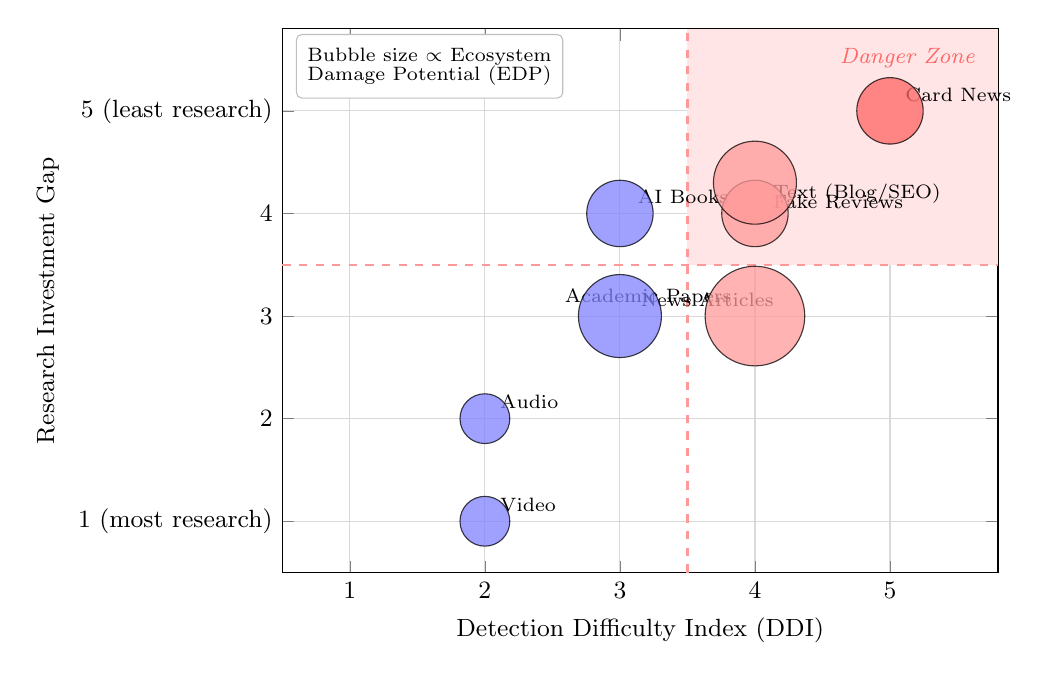
\begin{tikzpicture}
\begin{axis}[
    width=0.88\textwidth,
    height=0.70\textwidth,
    xlabel={Detection Difficulty Index (DDI)},
    ylabel={Research Investment Gap},
    xmin=0.5, xmax=5.8,
    ymin=0.5, ymax=5.8,
    xtick={1,2,3,4,5},
    ytick={1,2,3,4,5},
    yticklabels={1 (most research), 2, 3, 4, 5 (least research)},
    grid=major,
    grid style={gray!30},
    tick label style={font=\small},
    label style={font=\small},
    scatter/classes={
        fmt/.style={mark=*,draw=black,fill=blue!60,opacity=0.75}
    },
    clip=false,
]

% Danger zone shading (upper-right: DDI >= 3.5, Gap >= 3.5)
\fill[red!10] (axis cs:3.5,3.5) rectangle (axis cs:5.8,5.8);
\draw[red!40,dashed,thick] (axis cs:3.5,0.5) -- (axis cs:3.5,5.8);
\draw[red!40,dashed,thick] (axis cs:0.5,3.5) -- (axis cs:5.8,3.5);
\node[red!60,font=\footnotesize\itshape,anchor=north east] at (axis cs:5.7,5.7) {Danger Zone};

% Data points (sized by EDP: radius = 3 + EDP*3 pt)
% Video: DDI=2, Gap=1, EDP=2
\addplot[only marks, mark=*, mark size=9pt, fill=blue!50, draw=black, opacity=0.75]
    coordinates {(2,1)};
\node[font=\scriptsize,anchor=south west,xshift=2pt] at (axis cs:2,1) {Video};

% Audio: DDI=2, Gap=2, EDP=2
\addplot[only marks, mark=*, mark size=9pt, fill=blue!50, draw=black, opacity=0.75]
    coordinates {(2,2)};
\node[font=\scriptsize,anchor=south west,xshift=2pt] at (axis cs:2,2) {Audio};

% News Articles: DDI=3, Gap=3, EDP=4
\addplot[only marks, mark=*, mark size=15pt, fill=blue!50, draw=black, opacity=0.75]
    coordinates {(3,3)};
\node[font=\scriptsize,anchor=south west,xshift=4pt] at (axis cs:3,3) {News Articles};

% AI Books: DDI=3, Gap=4, EDP=3
\addplot[only marks, mark=*, mark size=12pt, fill=blue!50, draw=black, opacity=0.75]
    coordinates {(3,4)};
\node[font=\scriptsize,anchor=south west,xshift=3pt] at (axis cs:3,4) {AI Books};

% Academic Papers: DDI=4, Gap=3, EDP=5
\addplot[only marks, mark=*, mark size=18pt, fill=red!40, draw=black, opacity=0.75]
    coordinates {(4,3)};
\node[font=\scriptsize,anchor=south east,xshift=-5pt] at (axis cs:4,3) {Academic Papers};

% Text (Blog/SEO): DDI=4, Gap=4, EDP=3
\addplot[only marks, mark=*, mark size=12pt, fill=red!40, draw=black, opacity=0.75]
    coordinates {(4,4)};
\node[font=\scriptsize,anchor=south west,xshift=3pt] at (axis cs:4,4) {Text (Blog/SEO)};

% Fake Reviews: DDI=4, Gap=4, EDP=4
\addplot[only marks, mark=*, mark size=15pt, fill=red!40, draw=black, opacity=0.75]
    coordinates {(4,4.3)};
\node[font=\scriptsize,anchor=north west,xshift=3pt,yshift=-1pt] at (axis cs:4,4.3) {Fake Reviews};

% Card News: DDI=5, Gap=5, EDP=3
\addplot[only marks, mark=*, mark size=12pt, fill=red!60, draw=black, opacity=0.75]
    coordinates {(5,5)};
\node[font=\scriptsize,anchor=south west,xshift=2pt] at (axis cs:5,5) {Card News};

% Legend for bubble size
\node[font=\scriptsize,anchor=north west,draw=gray!50,fill=white,inner sep=4pt,rounded corners=2pt]
    at (axis cs:0.6,5.75) {%
    \begin{tabular}{@{}l@{}}
    Bubble size $\propto$ Ecosystem\\[-1pt]
    Damage Potential (EDP)
    \end{tabular}};

\end{axis}
\end{tikzpicture}
\caption{The Production--Detection Paradox (organizing hypothesis). Detection Difficulty Index (DDI, x-axis) is reproduced from the AMSM matrix. The Research Investment Gap (y-axis, inverted scale: 5\,=\,least research) is a \emph{preliminary expert estimate awaiting bibliometric validation under H2}; numeric positions on the y-axis encode the author's literature-volume reading and are explicitly subject to revision. Bubble size is proportional to Ecosystem Damage Potential (EDP). The shaded upper-right region marks the ``danger zone''---formats that are hard to detect, under-researched (under the current estimate), and cause significant harm. Points in the danger zone are shaded in red; points outside in blue.}
\label{fig:paradox}
\end{figure}

The formats in the danger zone are characterized by a triple deficit: they are easy to produce, hard to detect, and unstudied. This is the core of the paradox.

\subsection{Three Hypotheses for Why the Paradox Exists}

Why has research investment been directed toward the least-threatening format? Three hypotheses follow.

\textbf{Visibility bias.} Video slop is visually striking---AI-generated animals with impossible anatomy, celebrity deepfakes, surreal landscapes---and makes compelling demonstrations in media coverage, conference presentations, and public discourse. Text slop, by contrast, is designed to be invisible. It reads fluently, uses proper grammar, and presents plausible-sounding information. The very quality that makes text slop dangerous (its undetectability) makes it uninteresting as a research showcase.

\textbf{Methodological path dependence.} Deepfake detection research predates the AI slop era by several years, with FaceForensics++ (2019) and the Deepfake Detection Challenge (2020) establishing benchmarks, datasets, and a research community. When ``AI slop'' emerged as a concern in 2024--2025, this existing infrastructure made video the natural entry point for researchers. Text detection research exists but is framed as ``AI-generated text detection'' rather than ``slop detection''---a distinction that matters because AI-generated text is not inherently slop, and the quality dimension is underexplored.

\textbf{Platform disclosure asymmetry.} Platforms are more transparent about video content than text content. YouTube publishes trending data, provides a research API, and makes algorithmic recommendations visible to researchers. Text-based platforms (search engines, review sites, social media posts) provide far less research access. Instagram's API restrictions, Coupang's lack of any research API, and Naver's limited data sharing create an information asymmetry that channels research toward video.

\subsection{Implications of the Paradox}

The Production--Detection Paradox has three implications for the field.

\textbf{Research reallocation.} Funding agencies and researchers should prioritize formats in the danger zone---particularly hybrid image-text formats, adversarial-robust text detection, and non-English language detection. The creation of the first card news/infographic detection benchmark would, by itself, constitute a major contribution.

\textbf{Detection evaluation standards.} All detection research should include adversarial robustness testing as a standard requirement, not an optional addition. Benchmark results without adversarial evaluation dramatically overstate real-world performance, particularly for text.

\textbf{Policy reframing.} Regulators should decouple ``most visible'' from ``most harmful.'' Current AI labeling mandates, by focusing on ``content that is difficult to distinguish from reality'' (Korea AI Basic Act), implicitly target video and audio while leaving text---which is by definition difficult to distinguish from human writing---largely uncovered.


% ============================================================
% 5  THE ALGORITHM-SLOP CO-EVOLUTION MODEL
% ============================================================
\section{The Algorithm--Slop Co-evolution Model}
\label{sec:coevolution}

\subsection{Beyond Distribution}

The conventional framing treats platform algorithms as distribution channels for slop---neutral pipes through which low-quality content flows. This framing is inadequate. The evidence reviewed in this paper, combined with emerging research on recommender system feedback loops, supports a more dynamic model: algorithms and slop co-evolve, each shaping the other in a reinforcing cycle.

The co-evolution model differs from established filter bubble and echo chamber frameworks \parencite{Pariser2011,Sunstein2017} in three ways. First, it operates at the \emph{ecosystem} level rather than the individual level---the feedback loop shapes the overall content composition of a platform, not just an individual user's exposure. Second, it includes an economic validation stage that closes the loop through creator revenue, a mechanism absent from attention-focused models. Third, it generates format-specific predictions: the cycle velocity should vary by production cost, with text and card news completing the loop faster than video.

This framing draws on several theoretical foundations. \textcite{Simon1971}'s attention economy theory established that information abundance creates attention scarcity, and that the allocation of scarce attention is determined by systems that select and filter information. In digital platforms, these systems are recommendation algorithms optimized for engagement. \textcite{Grimmelmann2009}'s application of Gresham's Law to digital content---``bad content drives out good''---predicts that when consumers cannot distinguish quality, low-cost production dominates. \textcite{MadsenPuyt2025} extended this to AI slop specifically: ``monetization programs actively reward volume over value.'' Platform capitalism theory \parencite{Srnicek2017} emphasizes that platforms are not neutral infrastructure but economic actors whose revenue depends on maximizing engagement, creating structural incentives aligned with slop production.

The empirical evidence for feedback loops in recommendation systems is substantial. \textcite{Baumann2026}, auditing TikTok with bot accounts, found rapid reinforcement: within the first 200 videos, the algorithm strongly amplified interest-matching content, with a strong negative correlation between amplification and content diversity. \textcite{Mansoury2020} demonstrated through simulation that recommendation algorithms create feedback loops producing ascending popularity bias, declining aggregate diversity, and progressive user homogenization---with disproportionate impact on minority-group users. \textcite{Shumailov2024} showed a complementary mechanism at the training level: AI models trained on recursively generated data undergo ``model collapse,'' with output distributions progressively narrowing. A mathematical model of attention economy co-evolution \parencite{LiZhang2026} demonstrated that ``when the audience's ability to distinguish content quality is weak, selective attention and high-quality production simultaneously disappear, leading to informational collapse.''

\subsection{The Four-Stage Co-evolution Cycle}

\begin{figure}[htbp]
\centering
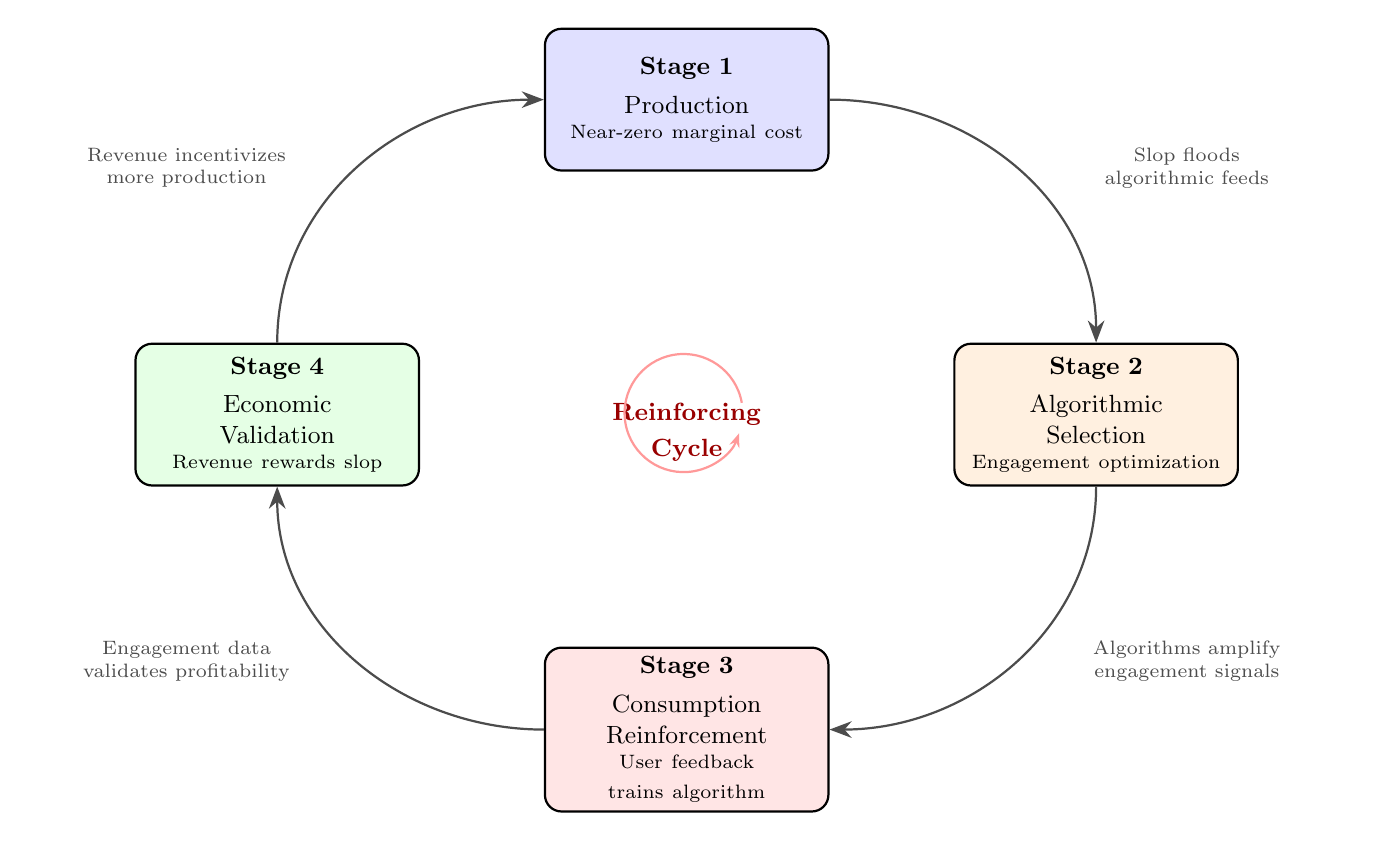
\begin{tikzpicture}[
    stage/.style={
        draw=black, thick, rounded corners=6pt,
        minimum width=3.6cm, minimum height=1.8cm,
        text width=3.2cm, align=center, font=\small,
        fill=#1
    },
    arrow/.style={
        -{Stealth[length=8pt,width=6pt]}, thick, black!70
    },
    desc/.style={
        font=\scriptsize, text width=3.8cm, align=center, black!70
    }
]

% Nodes in a circular (diamond) layout
\node[stage=blue!12] (prod) at (0,4)
    {\textbf{Stage 1}\\\smallskip Production\\[-2pt]{\scriptsize Near-zero marginal cost}};

\node[stage=orange!12] (algo) at (5.2,0)
    {\textbf{Stage 2}\\\smallskip Algorithmic\\Selection\\[-2pt]{\scriptsize Engagement optimization}};

\node[stage=red!10] (cons) at (0,-4)
    {\textbf{Stage 3}\\\smallskip Consumption\\Reinforcement\\[-2pt]{\scriptsize User feedback trains algorithm}};

\node[stage=green!10] (econ) at (-5.2,0)
    {\textbf{Stage 4}\\\smallskip Economic\\Validation\\[-2pt]{\scriptsize Revenue rewards slop}};

% Curved arrows connecting stages
\draw[arrow] (prod.east) to[out=0,in=90]
    node[desc,pos=0.5,right,xshift=4pt] {Slop floods\\algorithmic feeds}
    (algo.north);

\draw[arrow] (algo.south) to[out=-90,in=0]
    node[desc,pos=0.5,right,xshift=4pt] {Algorithms amplify\\engagement signals}
    (cons.east);

\draw[arrow] (cons.west) to[out=180,in=-90]
    node[desc,pos=0.5,left,xshift=-4pt] {Engagement data\\validates profitability}
    (econ.south);

\draw[arrow] (econ.north) to[out=90,in=180]
    node[desc,pos=0.5,left,xshift=-4pt] {Revenue incentivizes\\more production}
    (prod.west);

% Central reinforcing label
\node[font=\small\bfseries,text=red!60!black] at (0,0) {Reinforcing};
\node[font=\small\bfseries,text=red!60!black] at (0,-0.45) {Cycle};

% Circular arrow in center to indicate loop
\draw[red!40, thick, -{Stealth[length=5pt]}] (0.7,0.15) arc[start angle=10,end angle=340,radius=0.75cm];

\end{tikzpicture}
\caption{The Algorithm--Slop Co-evolution Feedback Loop. Four stages form a reinforcing cycle: mass production of slop (Stage~1) feeds algorithmic selection systems optimized for engagement (Stage~2), which amplifies slop to users whose engagement trains the algorithm to recommend more slop (Stage~3), generating ad revenue that validates and incentivizes further production (Stage~4). The cycle accelerates with each iteration, and its velocity is format-dependent---text and card news complete the loop fastest due to near-zero production costs.}
\label{fig:coevolution}
\end{figure}

\textbf{Stage 1: Production.} Near-zero marginal cost enables mass slop production. A ChatGPT subscription (\$20/month) can generate unlimited blog posts. Canva's Bulk Create produces 100 card news posts in 5 minutes. AI video generation, while more expensive, is dropping rapidly. The production barrier determines the entry velocity: text and card news enter the cycle fastest, video enters more slowly.

\textbf{Stage 2: Algorithmic Selection.} Engagement-optimized algorithms systematically favor slop. Slop is engineered for the metrics algorithms reward: high click-through rates (curiosity-gap thumbnails), high completion rates (short, stimulating content), and high interaction rates (emotionally provocative framing). The Kapwing cold-start experiment demonstrates this: new accounts with no history received 21\% AI slop after the algorithm began optimizing, up from 0\% in the first 16 recommendations. As \textcite{SEJ2026} observed: ``AI slop is taking over YouTube, and the algorithm is doing exactly what it was built to do.''

\textbf{Stage 3: Consumption Reinforcement.} User engagement with slop trains the algorithm to recommend more slop. \textcite{Baumann2026}'s TikTok audit showed rapid reinforcement within 200 videos. This creates path dependency: a single early engagement with slop biases future recommendations, creating what users describe as ``I liked one video and now I'm trapped in AI slop'' \parencite{Dexerto2026}. The critical insight from \textcite{Moller2026}---that AI content produces a ``negative spill-over effect'' on non-AI conversations---suggests that consumption reinforcement degrades not just individual feeds but entire platform environments.

\textbf{Stage 4: Economic Validation.} Ad revenue flows to slop channels, reinforcing production incentives. The 278 AI slop channels identified by Kapwing generated an estimated \$117 million annually. In Korea, AI slop channels earned approximately 170 billion KRW (\$130 million). The economic validation closes the loop: producers see evidence that slop is profitable, invest more in production, and the cycle accelerates.

The cycle then returns to Stage~1 at a larger scale. Each iteration increases the volume of slop in the ecosystem, trains algorithms on more slop-contaminated data, and raises the economic incentive for production.

\subsection{Natural Experiments Testing the Co-evolution Model}

The 2025--2026 period offers an unprecedented set of natural experiments, each disrupting the co-evolution cycle at a different stage:

\begin{table}[H]
\centering
\caption{Natural experiments testing the co-evolution model.}
\label{tab:experiments}
\small
\begin{tabularx}{\textwidth}{@{}l l c X @{}}
\toprule
\textbf{Natural Experiment} & \textbf{Date} & \textbf{Stage} & \textbf{Observable Outcome} \\
\midrule
Sora app shutdown & 2026.03.24 & 1 & Does removing a major production tool reduce AI video slop volume? \\
Instagram authentic content shift & 2026.01 & 2 & Does algorithmic demotion reduce slop exposure? \\
YouTube ``AI slop?'' feedback & 2026.03 & 3 & Does user feedback signal disrupt the reinforcement loop? \\
YouTube channel deletions & 2025--2026 & 4 & Does revenue removal reduce production incentives? \\
Korea AI labeling mandate & 2026.01.22 & 3--4 & Does transparency regulation alter consumption and economics? \\
\bottomrule
\end{tabularx}
\end{table}

Each experiment tests a specific causal claim. If the co-evolution model is correct, disrupting any single stage should produce a temporary reduction in slop followed by adaptation---producers finding alternative tools (Stage~1), gaming new algorithmic signals (Stage~2), exploiting user feedback mechanics (Stage~3), or migrating to unregulated platforms or formats (Stage~4). The adaptation prediction distinguishes the co-evolution model from a simpler linear model in which disrupting one stage would produce permanent reduction.

\subsection{Testable Hypotheses}

\textbf{H-CoEv1}: Engagement-optimized algorithms produce a measurable positive bias toward AI slop content relative to matched human content, controlling for topic, metadata, and posting time. \textit{Method}: Sock puppet algorithm audit with treatment (AI slop engagement) and control (matched human content engagement) conditions.

\textbf{H-CoEv2}: Platform interventions disrupting one stage of the co-evolution cycle produce a measurable but temporary reduction in slop metrics, with adaptation detectable within 3--6 months. \textit{Method}: Difference-in-differences analysis of Instagram content shift (Stage~2 disruption), YouTube channel deletions (Stage~4 disruption), and Sora shutdown (Stage~1 disruption).

\textbf{H-CoEv3}: The co-evolution cycle velocity---time from production to economic validation---is faster for formats with lower Production Cost Asymmetry. Text and card news slop should complete the cycle faster than video slop, observable as faster growth in volume following algorithmic amplification. \textit{Method}: Cross-format comparison of growth trajectories for new slop channels/accounts.


% ============================================================
% 6  RESEARCH AGENDA
% ============================================================
\section{Research Agenda}
\label{sec:agenda}

The AMSM framework, the Production--Detection Paradox, and the Algorithm--Slop Co-evolution Model together generate a research agenda organized by priority. Hypotheses are ranked by a combination of feasibility (data accessibility, methodological maturity) and impact (severity of the knowledge gap, policy relevance).

% TODO(review-2026-05-21,m1): For H-CoEv1 (sock puppet audit), specify the planned
%   n based on the Baumann 2026 / FAccT 2025 precedent of n=120 sock puppets; include
%   a power analysis (effect size detectable at n=120 vs. 240 vs. 60) before any
%   data collection.
% TODO(review-2026-05-21,m3): Pre-register H-Text, H-Prev, H-CoEv1-3, H-Adapt, H-Econ,
%   H-Spill on OSF before any data collection that has not yet started.
\subsection{Priority Hypotheses}

\begin{table}[H]
\centering
\caption{Research agenda: seven priority items. Items marked with \textsuperscript{\dag} are predictive hypotheses with explicit falsification conditions; item H-Gap is a literature-state claim with a constructive corollary (a benchmark whose absence is itself the testable artefact). Predictive hypotheses are intended for the family-wise correction policy described in the companion Perspectives paper.}
\label{tab:agenda}
\small
\begin{tabularx}{\textwidth}{@{}c X l l c c c @{}}
\toprule
\textbf{\#} & \textbf{Hypothesis / Priority} & \textbf{Format} & \textbf{Method} & \textbf{Feas.} & \textbf{Impact} & \textbf{Plat.?} \\
\midrule
1 & H-Gap (literature-state claim): No published detection method, as of the May 2026 literature snapshot, achieves AUROC $> 0.60$ on a curated hybrid image-text card-news benchmark; the constructive corollary is the first such benchmark. \textit{Refuted if:} a published method achieving AUROC $> 0.60$ on hybrid image-text card-news content is identified. & Card News & Build first hybrid detection pipeline; document baseline failure of existing text/image detectors & Med & V.\ High & No \\
\addlinespace
2\textsuperscript{\dag} & H-Text: Text detection falls below useful thresholds under adversarial conditions while video detection remains above 0.70 & Text vs.\ Video & Adversarial benchmark evaluation & High & V.\ High & No \\
\addlinespace
3\textsuperscript{\dag} & H-Prev: AI text penetration exceeds AI video penetration by $\geq$\,2$\times$ & Text vs.\ Video & Web crawl + video feed audit & High & High & No \\
\addlinespace
4\textsuperscript{\dag} & H-CoEv1: Algorithms exhibit measurable positive bias toward AI slop & All (Shorts) & Sock puppet audit & Med & High & No \\
\addlinespace
5\textsuperscript{\dag} & H-Adapt: Interventions produce $<$\,6 months of disruption before adaptation & Video, Image & DiD analysis of 2026 interventions & High & High & Partial \\
\addlinespace
6\textsuperscript{\dag} & H-Econ: AI slop produces measurable economic displacement of authentic creators & Video, Text & Social Blade data + creator surveys & Med & V.\ High & Partial \\
\addlinespace
7\textsuperscript{\dag} & H-Spill: Cross-format contamination pipeline exists (academic $\to$ news $\to$ blog) & Text (multi) & Citation/content tracing & Med & High & No \\
\bottomrule
\end{tabularx}
\end{table}

\subsection{What Independent Researchers Can Do}

A meaningful portion of this agenda is accessible to independent researchers without institutional affiliation or platform partnerships:

\textbf{Algorithm audits} via sock puppet methodology are the single most impactful tool available to independent researchers. \textcite{Baumann2026} and FAccT 2025 X/Twitter audits (120 sock puppets) demonstrate established methodology. The technical requirements---browser automation, account management, data logging---are within the capabilities of an independent developer.

\textbf{Web crawl-based text slop prevalence studies} require only a web crawler, detection tools (GPTZero API, Originality.AI API, KatFishNet), and a sampling framework. Ahrefs' 900,000-page analysis and Originality.AI's Google Search results tracking provide methodological precedents.

\textbf{Card news detection gap documentation}---simply demonstrating that no detection tool can handle this format---requires testing existing tools against a manually curated set of known-AI and known-human card news posts. The result, even if negative (tools fail), would constitute a publication-worthy finding that establishes the gap.

\textbf{Natural experiment analysis} of publicly observable events (Instagram content shift, YouTube feedback system, Sora shutdown, Korean regulation) requires only time-series data collection before and after the event, accessible through platform APIs and tools such as Social Blade.

\subsection{What Requires Platform Cooperation}

Certain questions cannot be answered without internal platform data:

\textbf{True algorithmic recommendation rates}---what percentage of impressions go to AI slop---are knowable only from internal platform dashboards. External sock puppet audits provide estimates but cannot achieve the precision of internal data.

\textbf{Content moderation outcome data}---removal rates, appeal rates, false positive/negative rates by format---are held exclusively by platforms.

\textbf{A/B testing of intervention designs}---the gold standard for evaluating whether a specific algorithmic change reduces slop---requires platform engineering resources.

The research community should advocate for platform transparency mechanisms that make these data accessible for research, as proposed by the EU's Digital Services Act and supported by academic coalitions.

\subsection{The Most Critical Gap: Card News and Hybrid Formats}

If this paper generates one research response, it should be the construction of the first card news/infographic AI slop detection benchmark. This format scores 5 (maximum) on three of five AMSM dimensions (DDI, AAS, RCG), scores 5 on Production Cost Asymmetry, and has received zero academic attention. It is a major information format on widely used platforms including Instagram, Facebook, Naver, and KakaoTalk. In Korea specifically, card news is a culturally distinct format---described as ``the first `dominant' multimedia format in Korean media history'' \parencite{Bae2018}---with a production pipeline that has been fully automated by AI tools. The absence of any detection research for this format represents a failure of the field to match its attention to the actual landscape of AI content pollution.


% ============================================================
% 7  IMPLICATIONS
% ============================================================
\section{Implications}
\label{sec:implications}

\subsection{For Platforms}

Content moderation must become format-aware. The current approach---treating ``AI content'' as a homogeneous category addressed primarily through video-focused detection---misses the majority of AI slop. The AMSM framework suggests that platforms should allocate moderation resources proportionally to composite threat scores, which would shift investment from video (composite 2.6) toward text (3.8), reviews (3.8), and especially hybrid formats such as card news (4.6).

Engagement optimization is the structural driver of the co-evolution cycle. As \textcite{MadsenPuyt2025} argue, platforms that ``reward volume over value'' are ``industrial slop farms'' by design. Breaking the co-evolution cycle at Stage~2 (Algorithmic Selection) requires changing the objective function of recommendation algorithms---a technically feasible but commercially costly intervention that trades short-term engagement for long-term ecosystem health.

Cold-start conditions deserve specific attention. The Kapwing finding that new accounts are disproportionately exposed to slop (21--33\%) suggests that the algorithms' popularity-based fallback during cold start is particularly vulnerable. Cold-start slop exposure audits should be standard platform practice.

\subsection{For Regulators}

Current AI labeling mandates are disproportionately video-biased. The Korea AI Basic Act's focus on content that is ``difficult to distinguish from reality'' implicitly targets visual media; text content---which is by definition difficult to distinguish from human writing---is paradoxically under-covered. The EU AI Act's Article~50 transparency provisions should be evaluated for format coverage breadth.

Format-specific enforcement is needed. The FTC's fake review rule (\$51,744 per violation) is a model for format-specific regulation, but its enforcement has been minimal \parencite{FTC2024}. Similar mechanisms for AI-generated news, card news, and academic content would address the AMSM-identified gaps.

Detection tool accuracy claims should be independently verified before regulatory reliance. The FTC itself has warned that detection tool providers exaggerate accuracy; relying on tools with 88--95\% benchmark performance that drops to 60--70\% in real conditions (and to AUROC 0.43 under adversarial attack) would produce unreliable enforcement.

\subsection{For Researchers}

The Production--Detection Paradox is a call for research reallocation. The field should diversify beyond video to address text (especially under adversarial conditions), hybrid formats (where zero research exists), and non-English languages (where detection tools are scarce and perform poorly). Every detection paper should include adversarial robustness evaluation as standard methodology.

Cross-format comparison studies---enabled by AMSM or similar frameworks---should become a research priority. Studying each format in isolation prevents the field from understanding relative threat levels, allocating resources effectively, or identifying cross-format contamination pipelines.

The co-evolution model generates testable hypotheses via natural experiments. The concentration of platform interventions and regulatory changes in 2025--2026 creates a time-limited window for difference-in-differences and regression discontinuity designs that may not recur.

\subsection{For the Public}

Media literacy education has focused overwhelmingly on deepfake video---teaching people to look for visual artifacts, unnatural lip sync, and impossible physics. This is necessary but insufficient. The AMSM framework suggests that the most dangerous forms of AI slop are invisible by design: text that reads naturally, reviews that sound genuine, card news that looks professional, academic papers that follow proper formatting.

``Your AI slop bores me''---the viral catchphrase of early 2026---captures legitimate fatigue with visible slop. But the slop that should worry us most is the kind we never notice.


% ============================================================
% 8  LIMITATIONS
% ============================================================
\section{Limitations}
\label{sec:limitations}

This section acknowledges several limitations of the AMSM framework and the analyses presented in this paper.

\textbf{AMSM scoring subjectivity.} The 1--5 ratings in the AMSM matrix involve expert judgment. While each score is grounded in cited evidence, alternative rating schemes are plausible. The composite score uses unweighted means; different weighting schemes (e.g., prioritizing EDP for policy applications or DDI for technical applications) would produce different rankings. Future research should explore inter-rater reliability with multiple expert panels to assess the stability of these ratings.

\textbf{Sensitivity analysis.} A sensitivity analysis varying dimension weights demonstrates that card news retains its top-3 position across all tested weighting schemes, but the relative ordering of text, reviews, and academic papers shifts depending on whether EDP or DDI receives higher weight. Future work should explore stakeholder-driven weighting through Delphi methods.

\textbf{Temporal validity.} The AMSM ratings reflect conditions as of March 2026. Detection capabilities, platform policies, and production tools evolve rapidly. DDI scores in particular may change significantly as detection research progresses---card news DDI\,=\,5 reflects the current absence of detection tools, not an inherent undetectability. Periodic re-evaluation of the matrix is essential as the landscape shifts.

\textbf{Industry report dependence.} Several data points (Kapwing, Originality.AI, Social Blade) come from industry sources with commercial interests. While these provide the best available data in a rapidly evolving field, peer-reviewed validation of key metrics is needed. Where possible, this paper has triangulated industry data with peer-reviewed studies (e.g., \textcite{Jones2025}; \textcite{Moller2026}), but certain claims---particularly prevalence estimates---rest on single industry sources.

\textbf{Geographic scope.} While this paper draws on evidence from multiple jurisdictions (US, EU, Korea, China), the card news analysis draws disproportionately on the Korean context. Whether the card news phenomenon generalizes to other markets with similar platform structures (e.g., LINE in Japan, Zalo in Vietnam) remains an empirical question.

\textbf{Practitioner positionality.} The author's background as an independent developer provides direct familiarity with production tools and pipelines, but this vantage point may introduce blind spots regarding institutional research dynamics or regulatory processes. The production cost estimates, while grounded in documented tool capabilities, have not been independently validated through controlled studies.

\textbf{Format boundary ambiguity.} Content formats are not discrete categories. A blog post may embed card news; a news article may be reposted as an Instagram carousel; an academic paper may be summarized as a TikTok video. The AMSM framework treats formats independently, but cross-format transformation pipelines (addressed in H-Spill) require further theoretical development.

\textbf{Single-author circularity in H2 testing.} When the bibliometric protocol pre-registered for H2 (\S\ref{sec:agenda}; see also \texttt{experiments/h2\_misallocation/protocol.md} in the project repository) is executed, it correlates publication counts against the AMSM PDA scores published in this paper. Because both inputs originate from the same author, a finding consistent with H2 establishes \emph{internal consistency} between this author's qualitative reading of the format landscape and the external bibliometric record, not a test against an independently constructed ground-truth ranking. A multi-rater AMSM (e.g., Delphi panel) followed by re-running H2 against the panel-mean PDA scores would be required to factor out single-author judgment as a confound.

\textbf{Dual-use risk of the framework.} The AMSM matrix and the Production--Detection Paradox jointly identify, for any adversarial reader, the formats at which detection investment is currently weakest and where slop production is therefore most likely to evade response. Card news in particular is named as the format with the largest detection gap. This paper proceeds on the judgment that the dual-use risk of \emph{naming} the gap is outweighed by the policy and research benefit of making the misallocation legible, given that the production economics of these formats are already widely known among practitioners and slop-pipeline vendors (see \S\ref{sec:amsm}). Future versions of this work should consider partitioning the most operationally sensitive findings (e.g., detailed adversarial-attack budgets per format) into a separate venue with restricted distribution.


% ============================================================
% 9  CONCLUSION
% ============================================================
\section{Conclusion}
\label{sec:conclusion}

This paper has argued that the video-centric framing of AI slop is both incomplete and counterproductive. By proposing the AI-Generated Multi-Format Slop Model (AMSM), it provides the first unified framework for comparing AI slop across content formats on five operationalizable dimensions: Production Cost Asymmetry, Detection Difficulty Index, Ecosystem Damage Potential, Algorithmic Amplification Susceptibility, and Regulatory Coverage Gap.

The application of AMSM reveals that the formats receiving the most attention---video and audio---are the most detectable, the most regulated, and the least systemically damaging. Meanwhile, text-based formats (blogs, SEO spam, fake reviews, academic papers, news articles) cluster in a region of high production scalability and high detection difficulty. And hybrid image-text formats (card news, infographics, carousel posts)---which dominate social media engagement metrics and serve as a culturally central information format in several major markets---have received zero detection research.

The Production--Detection Paradox formalizes this misallocation: research investment is inversely correlated with actual threat, driven by visibility bias, methodological path dependence, and platform disclosure asymmetry. The Algorithm--Slop Co-evolution Model reframes the relationship between platforms and slop as a dynamic feedback system in which algorithms and slop mutually reinforce each other through production, selection, consumption, and economic validation stages---a system that can be empirically tested through the natural experiments of 2025--2026.

The research agenda proposed here is not merely theoretical. Seven hypotheses are specified with methods, feasibility assessments, and impact ratings. Several are executable by independent researchers without platform cooperation. The most urgent is the creation of the first hybrid-format detection benchmark, addressing the single largest gap in the field.

AI slop is not a video problem. It is an information ecosystem problem that spans every content format, from the 100 card news posts produced in five minutes to the 11,300 academic papers retracted from a single publisher. The AMSM framework offers a map of the full terrain. The field should use it.

\vspace{1em}
\noindent\textit{The author declares no conflicts of interest.}


% ============================================================
% REFERENCES
% ============================================================
\newpage
\printbibliography

\end{document}
